\documentclass[a4paper,10pt]{article}
\usepackage[utf8]{inputenc}
\usepackage[nottoc,numbib]{tocbibind} % makes the BibTeX references section appear in the table of contents
\usepackage[inline]{enumitem}
\usepackage{amssymb}
\usepackage{amsfonts}
\usepackage{amsmath}
\usepackage{amsthm}
\usepackage{color}
\usepackage{caption}
\usepackage{subcaption}
\usepackage{graphicx}
\usepackage{mathtools}
\usepackage{mathrsfs}
\usepackage{framed}
% eventually make left/right margins equal
\usepackage[top=0.6in,bottom=0.6in,left=0.6in,right=0.6in]{geometry}
\usepackage{dsfont}



\usepackage[textwidth=0.7in]{todonotes}

\usepackage[hidelinks]{hyperref} %this needs to be loaded last!

% for 3D pictures
\usepackage{tikz}
\usepackage{tikz-3dplot}
\usetikzlibrary{perspective}
\tdplotsetmaincoords{82}{20}

%prevent math mode statements from being broken up across lines
\relpenalty=9999
\binoppenalty=9999

%claim environment
\newenvironment{claim}[1]{\par\noindent\underline{Claim:}\space#1}{}

%leftbar
\renewenvironment{leftbar}[1][\hsize]
{%
    \def\FrameCommand
    {%
        {\vrule width 3pt}%
        \hspace{0pt}%must no space.
        \fboxsep=\FrameSep\colorbox{white}%
    }%
    \MakeFramed{\hsize#1\advance\hsize-\width\FrameRestore}%
}
{\endMakeFramed}


%numbering and style of theorems
\theoremstyle{plain}
\newtheorem{Theorem}{Theorem}
\newtheorem{Proposition}[Theorem]{Proposition}
\newtheorem{Corollary}[Theorem]{Corollary}
\newtheorem{Lemma}[Theorem]{Lemma}
\newtheorem{Question}[Theorem]{Question}
\newtheorem{Conjecture}[Theorem]{Conjecture}
\newtheorem{Assumption}[Theorem]{Assumption}
\newtheorem{Algorithm}[Theorem]{Algorithm}

\theoremstyle{definition}
\newtheorem{Definition}[Theorem]{Definition}
\newtheorem{Property}[Theorem]{Property}
\newtheorem{Notation}[Theorem]{Notation}
\newtheorem{Condition}[Theorem]{Condition}
\newtheorem{Example}[Theorem]{Example}
\newtheorem{Exercise}[Theorem]{Exercise}
\newtheorem{Introduction}[Theorem]{Introduction}

\theoremstyle{remark}
\newtheorem{Remark}[Theorem]{Remark}
\newtheorem{case}{Case}[Theorem]

% make proofs use filled in black square instead of empty square
\renewcommand{\qedsymbol}{$\blacksquare$}
%\renewcommand\proof{\noindent\textit{\textbf{Proof. }}}
\newcommand{\modo}[3]{#1 \equiv #2 \pmod{#3}}
\newcommand{\nmodo}[3]{#1 \not\equiv #2 \pmod{#3}}
\newcommand{\R}{\mathbb{R}}
\newcommand{\Q}{\mathbb{Q}}
\newcommand{\N}{\mathbb{N}}
\newcommand{\Z}{\mathbb{Z}}
\newcommand{\Zpos}{\mathbb{Z}_{\geq 0}}
\renewcommand{\vec}[1]{\textbf{#1}}
\newcommand{\dist}{\text{dist}}
\newcommand{\F}{\mathbb{F}}
\newcommand{\C}{\mathbb{C}}
\newcommand{\lin}{\text{lin}}
\newcommand{\cl}{\text{cl}}
\newcommand\norm[1]{\left\lVert#1\right\rVert}
\newcommand{\ONE}{\mathds{1}}
\newcommand{\generatedby}[1]{\left\langle#1\right\rangle}
\newcommand{\id}{\text{id}}
\DeclareMathOperator{\sgn}{sgn}
\newcommand\abs[1]{\left|#1\right|}
\newcommand\Gl{\text{Gl}}

\title{Icosahedral Virus Transitions: Computational Techniques \\ \large WMRUGS Talk: Paper Format}
\author{Xavier Silva}

\begin{document}
\maketitle
\tableofcontents

\section{Quick Summary}
Parallel computation allows for efficient identification of the symmetries that are preserved during maturation of icosahedral viruses.

\section{Group Theory}
Group theory is a subset of abstract algebra.
In particular, group theory studies the mathematical object known as a group, defined in definition \ref{def:group}.
\begin{Definition}[Group]
    \label{def:group}
    A group \(G\) is a set along with a binary operation \(*\) that satisfy the following properties:
    \begin{enumerate}
        \item Closure: If \(a, b \in G\), then \(a*b \in G\).
        \item Associativity: If \(a, b, c \in G\), then \((a*b)*c = a*(b*c)\).
        \item Identity: There exists \(e \in G\) such that \(a*e = e*a = a\) for all \(a \in G\).
        \item Inverses: For all \(a \in G\) there exists \(b \in G\) such that \(a*b = b*a = e\). Thus \(b = a^{-1}\).
    \end{enumerate}
\end{Definition}
Beyond the rigorous definition, groups can be thought of as symmetries of an object (one can think about this through group actions).
The idea of groups representing symmetry is crucial to understanding the structure of icosahedral viruses.

\subsection{Icosahedral Group}
The set of symmetries on an icosahedral virus is the icosahedral group \(\mathcal{I}\).
\begin{Definition}[Icosahedral Group]
    The icosahedral group, denoted by \(\mathcal{I}\), is the 60-element group given by \[\mathcal{I} := \generatedby{a, b | a^2 = b^3 = (ab)^5 = 1}\]
\end{Definition}
These viruses have 2-fold, 3-fold, and 5-fold symmetries, which relates to the structure of the icosahedral group.
We wish to investigate whether icosahedral symmetry is preserved during virus maturation.

\begin{figure}[h]
	\centering
	\captionsetup{width=0.5\textwidth}
	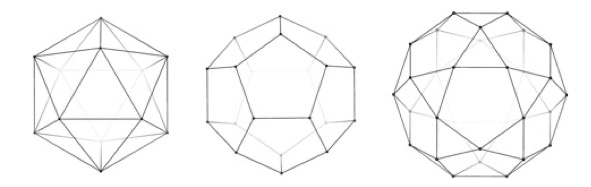
\includegraphics[width=0.5\textwidth]{images/ICO_DOD_IDD.jpg}
	\caption{Images of the icosahedron, dodecahedron, and icosidodecahedron.}
\end{figure}

\subsection{Realization of Icosahedral Group}
We realize icosahedral symmetry as a \( 6 \times 6 \) matrix group.
The operation matrix groups use is matrix multiplication.
\begin{Definition}[Generators of \(\mathcal{I}\)]
    The generators of \(\mathcal{I}\) are:
    \[a = \begin{bmatrix}
    -1 & 0  & 0 & 0 & 0 & 0 \\
    0  & -1 & 0 & 0 & 0 & 0 \\
    0  & 0  & 0 & 0 & 1 & 0 \\
    0  & 0  & 0 & 0 & 0 & 1 \\
    0  & 0  & 1 & 0 & 0 & 0 \\
    0  & 0  & 0 & 1 & 0 & 0
\end{bmatrix} \quad b = \begin{bmatrix}
    0 & -1 & 0  & 0 & 0 & 0 \\
    0 & 0  & -1 & 0 & 0 & 0 \\
    1 & 0  & 0  & 0 & 0 & 0 \\
    0 & 0  & 0  & 0 & 0 & 1 \\
    0 & 0  & 0  & 1 & 0 & 0 \\
    0 & 0  & 0  & 0 & 1 & 0
\end{bmatrix}.\]
\end{Definition}

\subsection{Maximal Subgroups of \(\mathcal{I}\)}
The icosahedral group has maximal subgroups \(A_4, D_{10}, \text{ and } D_6\).
\begin{itemize}
    \item \(A_4\) has multiple 2-fold and 3-fold axes.
    \item \(D_{6}\) has a singular 2-fold and 3-fold axis.
    \item \(D_{10}\) has a 5-fold and a 2-fold axis.
\end{itemize}
These are subsets of \(\mathcal{I}\) and more specificially, maximal subgroups of \(\mathcal{I}\).
Similar to how the icosahedral group represents the shape of an icosahedron, these maximal subgroups represent their own shapes.
These shapes are shown in figure \ref{fig:maximal_subgroups}.
We use these subgroups because if we are unable to preserve all of icosahedral symmetry, then we wish to at least preserve the symmetry of one of these maximal subgroups.
\begin{figure}[h]
	\captionsetup{width=0.75\textwidth}
	\centering
	% A4
	\begin{tikzpicture}[scale=0.5, tdplot_main_coords,
		declare function={b=5;h=4.33;l=15;}]
		\draw[fill=gray,fill opacity=0.3] (b/2,-l/2,0)  -- (0,-l/2,h) -- (-b/2,-l/2,0) -- cycle;
		% \draw (b/2,-l/2,0) -- (0, l-20, h/3);
		% \draw (0,-l/2,h) -- (0, l-20, h/3);
		% \draw (-b/2,-l/2,0) -- (0, l-20, h/3);
		\draw (b/2,-l/2,0) -- (0, 0, h/3);
		\draw (0,-l/2,h) -- (0, 0, h/3);
		\draw[dashed] (-b/2,-l/2,0) -- (0, 0, h/3);
		\draw[orange,dashed] (0,-l/2,h/3) -- (0,l/2,h/3); % center to center aka 3 fold
		\draw[orange] (0,-l/2-10,h/3) -- (0,-l/2,h/3);
		% \node[fill=orange, circle, inner sep=4pt] at (0,-l/2,h/3) {};
		\draw[blue, dashed] (0, -l/4, 4*h/6) -- (0,-l/2,0);
		\draw[blue] (0, -l/4, 4*h/6) -- (0, -l/4+1/8*l, {4*h/6+1/8*(2*h+3)});
		\draw[blue] (0,-l/2,0) -- (0,-l/2-1/10*l,{-1/10*(2*h+3)});
		
		%draw the axes
		% \draw[red] (0,0,0) -- (3,0,0) node[anchor=west]{$x$};
		% \draw[green] (0,0,0) -- (0,3,0) node[anchor=west]{$y$};
		% \draw[blue] (0,0,0) -- (0,0,3) node[anchor=west]{$z$};
	\end{tikzpicture}
	% D10
	\begin{tikzpicture}[scale=0.4, tdplot_main_coords,
		declare function={r=3;l=5;}]
		% \draw ({r*cos(0)}, l, {r*sin(0)}) -- ({r*cos(72)}, l, {r*sin(72)}) -- ({r*cos(144)}, l, {r*sin(144)}) -- ({r*cos(216)}, l, {r*sin(216)}) -- ({r*cos(288)}, l, {r*sin(288)});
		
		% front face
		\draw[fill=gray,fill opacity=0.3] ({r*cos(18)}, -l, {r*sin(18)}) -- ({r*cos(90)}, -l, {r*sin(90)}) -- ({r*cos(162)}, -l, {r*sin(162)}) -- ({r*cos(234)}, -l, {r*sin(234)}) -- ({r*cos(306)}, -l, {r*sin(306)}) -- cycle;
		
		% back face
		\draw ({r*cos(18)}, l, {r*sin(18)}) -- ({r*cos(18+72)}, l, {r*sin(18+72)});
		\draw[dashed] ({r*cos(90)}, l, {r*sin(90)}) -- ({r*cos(90+72)}, l, {r*sin(90+72)});
		\draw[dashed] ({r*cos(162)}, l, {r*sin(162)}) -- ({r*cos(162+72)}, l, {r*sin(162+72)});
		\draw ({r*cos(234)}, l, {r*sin(234)}) -- ({r*cos(234+72)}, l, {r*sin(234+72)});
		\draw ({r*cos(306)}, l, {r*sin(306)}) -- ({r*cos(306+72)}, l, {r*sin(306+72)});
		
		
		% connect front and back faces
		\draw ({r*cos(18)}, l, {r*sin(18)}) -- ({r*cos(18)}, -l, {r*sin(18)});
		\draw ({r*cos(90)}, l, {r*sin(90)}) -- ({r*cos(90)}, -l, {r*sin(90)});
		\draw[dashed] ({r*cos(162)}, l, {r*sin(162)}) -- ({r*cos(162)}, -l, {r*sin(162)});
		\draw[dashed] ({r*cos(234)}, l, {r*sin(234)}) -- ({r*cos(234)}, -l, {r*sin(234)});
		\draw ({r*cos(306)}, l, {r*sin(306)}) -- ({r*cos(306)}, -l, {r*sin(306)});
		
		% 2-fold axis
		\draw[blue] (0,0,r+2) -- (0,0,r);
		\draw[blue, dashed] (0,0,r) -- (0,0,-r);
		\draw[blue] (0,0,-r) -- (0,0,-r-1);
		
		% 5-fold axis
		\draw[orange, dashed] (0, l+2*r, 0) -- (0, -l, 0);
		\draw[orange] (0, -l, 0) -- (0, -l-3*r, 0);
		
		
		%draw the axes
		% \draw[red] (0,0,0) -- (3,0,0) node[anchor=west]{$x$};
		% \draw[green] (0,0,0) -- (0,3,0) node[anchor=west]{$y$};
		% \draw[blue] (0,0,0) -- (0,0,3) node[anchor=west]{$z$};
	\end{tikzpicture}
	% D6
	\begin{tikzpicture}[scale=0.4, tdplot_main_coords,
		declare function={b=5;h=4.33;l=15;}]
		\draw[dashed] (-b/2,-l/2,0) -- (-b/2,l/2,0) edge (b/2,l/2,0) -- (0,l/2,h);     
		\draw (b/2,l/2,0) -- (0,l/2,h) -- (0,-l/2,h);
		\draw[fill=gray,fill opacity=0.3] (b/2,-l/2,0)  -- (0,-l/2,h) -- (-b/2,-l/2,0);
		\draw (b/2,-l/2,0)  -- (b/2,l/2,0);
		\draw (b/2,-l/2,0)  --   (-b/2,-l/2,0);
		% \draw (0,-l/2,0)  --  (0,-l/2,h);
		\draw[orange,dashed] (0,-l/2,h/3) -- (0,l/2+5,h/3); % center to center aka 3 fold
		\draw[orange] (0,-l/2-10,h/3) -- (0,-l/2,h/3);
		% \node[fill=orange, circle, inner sep=3pt] at (0,-l/2,h/3) {};
		% \node[draw=orange, circle, inner sep=3pt] at (0,l/2,h/3) {};
		
		\draw[blue] (0,0,h+2) -- (0,0,h); % top to bottom aka 2 fold
		\draw[blue, dashed] (0,0,h) -- (0,0,-1.1); % top to bottom aka 2 fold
		\draw[blue] (0,0,-1.1) -- (0,0,-2);
		
		%draw the axes
		% \draw[red] (0,0,0) -- (3,0,0) node[anchor=west]{$x$};
		% \draw[green] (0,0,0) -- (0,3,0) node[anchor=west]{$y$};
		% \draw[blue] (0,0,0) -- (0,0,3) node[anchor=west]{$z$};
	\end{tikzpicture}
	\caption{A visual representation of the maximal subgroups. From left to right we have \(A_4\), \(D_{10}\), and \(D_6\). The two fold axes are labeled in blue while the 3 or 5 fold axis is labeled in orange.}
	\label{fig:maximal_subgroups}
\end{figure}

\section{Point Arrays and Lattices}
Icosahedral viruses are characterized by point arrays, which are a set of points in 3 dimensions.
\begin{Definition}[Icosahedral Point Array]
    Let \(\vec{t}, \vec{v}_1, \vec{v}_2, \dots, \vec{v}_n\) be 6 dimensional vectors.
    Then the icosahedral point array generated by these vectors is \[P = \mathcal{I}\vec{v}_1 \cup \mathcal{I}\vec{v}_2 \cup \dots \cup \mathcal{I}\vec{v}_n \cup (\mathcal{I}\vec{v}_1 + \mathcal{I}\vec{t}) \cup (\mathcal{I}\vec{v}_2 + \mathcal{I}\vec{t}) \cup \dots \cup (\mathcal{I}\vec{v}_n + \mathcal{I}\vec{t}).\]
\end{Definition}
Notice that while icosahedral viruses are characterized by 3 dimensional point arrays, \emph{icosahedral point arrays} are 6 dimensional.
This is because we want icosahedral point arrays to fit inside icosahedral lattices, and no such lattices exist in dimensions lower than 6.\footnote{Because lattices of dimension 5 and lower cannot preserve 5-fold symmetry.}
However, we can project icosahedral point arrays from 6 dimensions into 3 dimensions using the projection matrix given in \cite{indelicatoetal2012}.

There are 55 standard point arrays from which we build all others.
These are called the \emph{one-base} point arrays and take the form \(\mathcal{I}\vec{v} \cup (\mathcal{I}\vec{v} + \mathcal{I}\vec{t})\). This form tells us that only one translation vector and one ``base" vector is needed to create the point array. \cite{keeftwarock2009affine}

\subsection{Constructing Point Arrays}
Constructing a one-base point array involves us finding all vectors in the set \(\mathcal{I}\vec{v} \cup (\mathcal{I}\vec{v} + \mathcal{I}\vec{t})\).
This is shown visually in figure \ref{fig:point_array_construction}.

\begin{figure}[h]
	\centering
	\begin{subfigure}{0.25\textwidth}
		\centering
		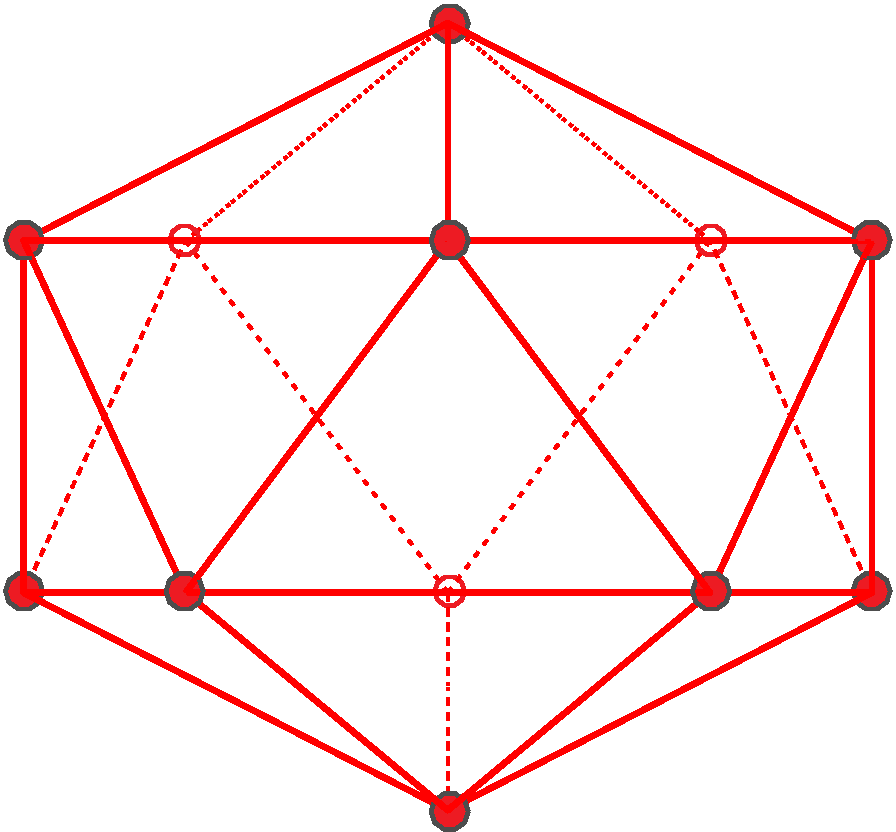
\includegraphics[width=\textwidth]{images/p_arr_construction_1.pdf}
		\caption{Start with icosahedron, created by applying icosahedral symmtry on one vector. Mathematically this is \(\mathcal{I}\vec{v}\).}
	\end{subfigure}
	\hfill
	\begin{subfigure}{0.3\textwidth}
		\centering
		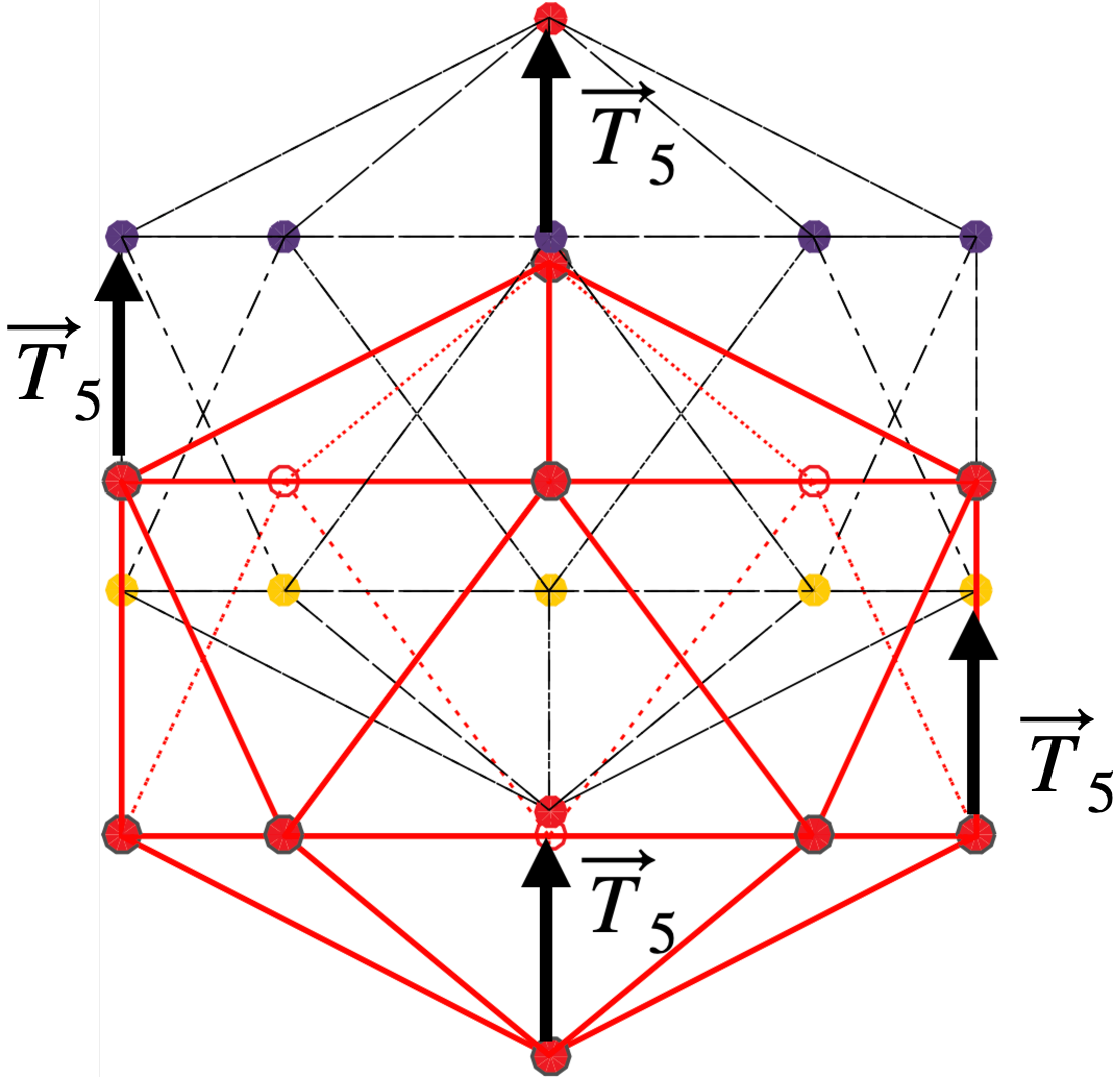
\includegraphics[width=\textwidth]{images/p_arr_construction_2.pdf}
		\caption{Shift icosahedron by a translation vector. Mathematically this is \mbox{\(\mathcal{I}\vec{v} \cup (\mathcal{I}\vec{v} + \vec{t})\)}.}
	\end{subfigure}
	\hfill
	\begin{subfigure}{0.35\textwidth}
		\centering
		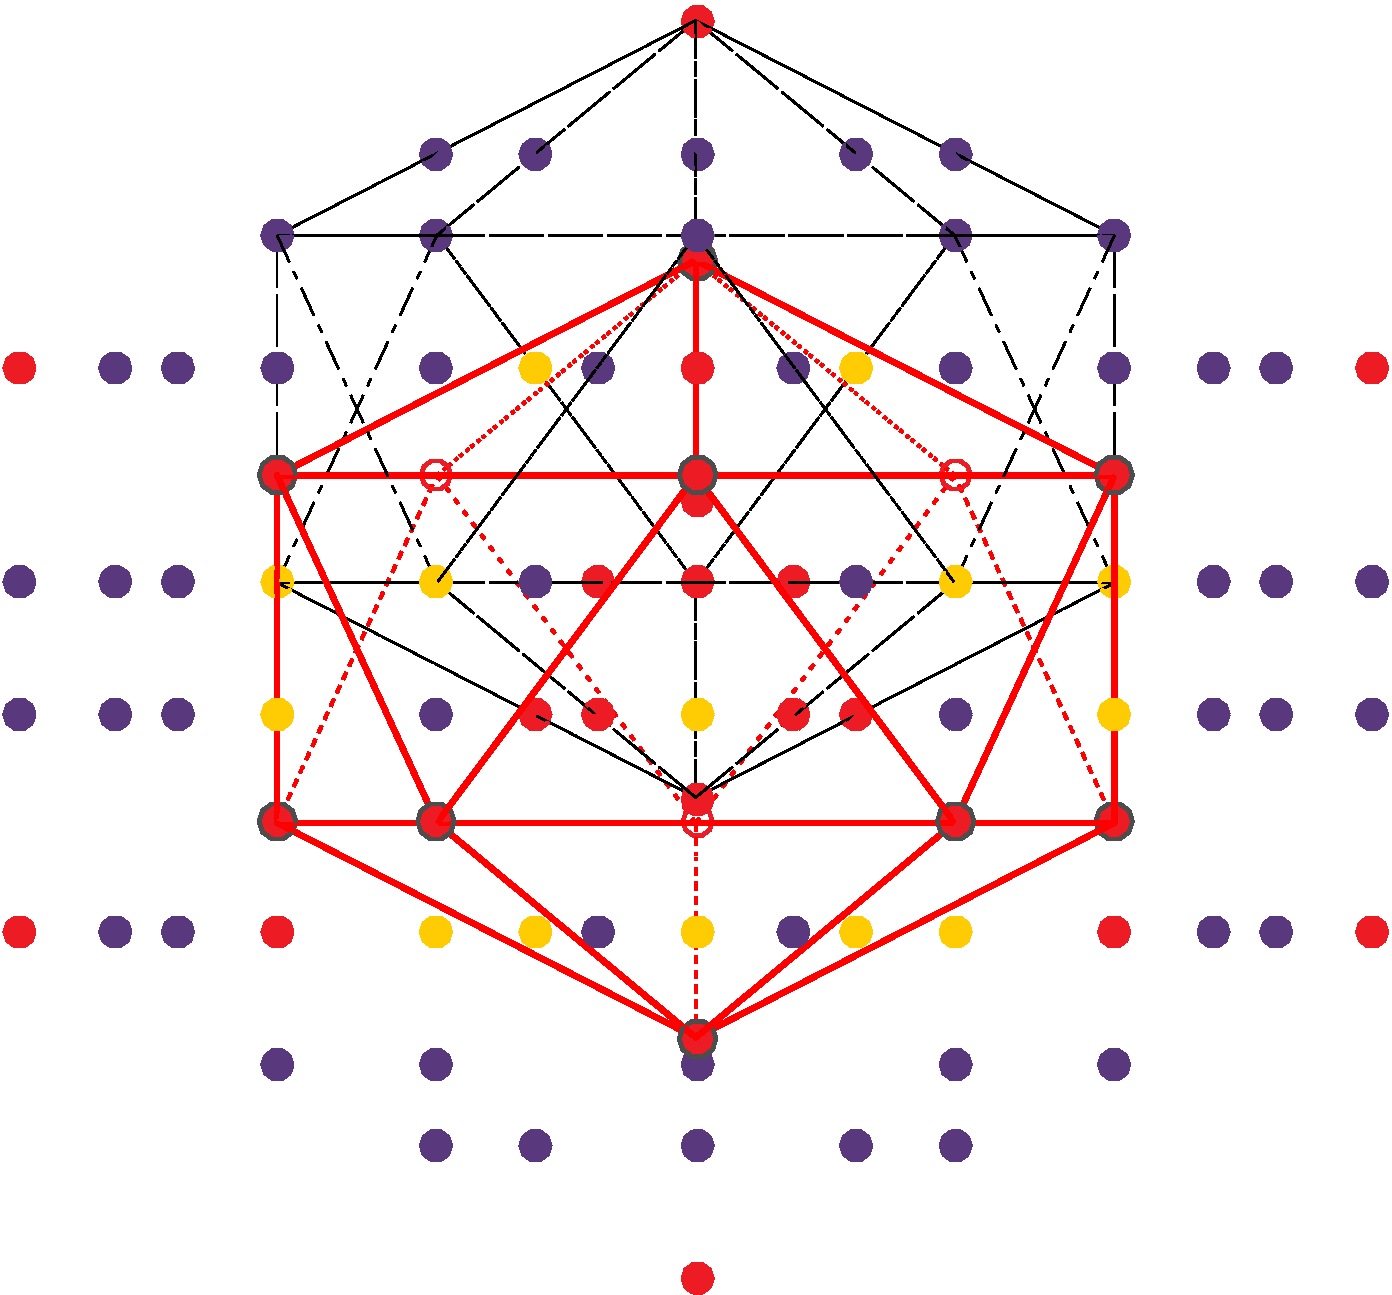
\includegraphics[width=\textwidth]{images/p_arr_construction_3.pdf}
		\caption{Reapply icosahedral symmetry, getting the final expression \(\mathcal{I}\vec{v} \cup (\mathcal{I}\vec{v} + \mathcal{I}\vec{t})\).}
	\end{subfigure}
	\caption{The process of creating a one-base point array.}
	\label{fig:point_array_construction}
\end{figure}

\section{Viral Maturation}
Icosahedral viruses mature over time, and maturation is how they become infectous.
For this paper we will focus on the Cowpea Chlorotic Mottle Virus (CCMV).
This virus is characterized by one of the standard point arrays.
How CCMV matures is shown by figure \ref{fig:CCMV_maturation}.
Notice the points in orange, these points collectively are the point arrays that characterize the CCMV virus.
We wish to see if there exists a linear transformation that maps the native point array to the mature point array while preserving icosahedral symmetry (or one of its maximal subgroups).

\begin{figure}[!h]
	\centering
	\captionsetup{width=0.5\textwidth}
	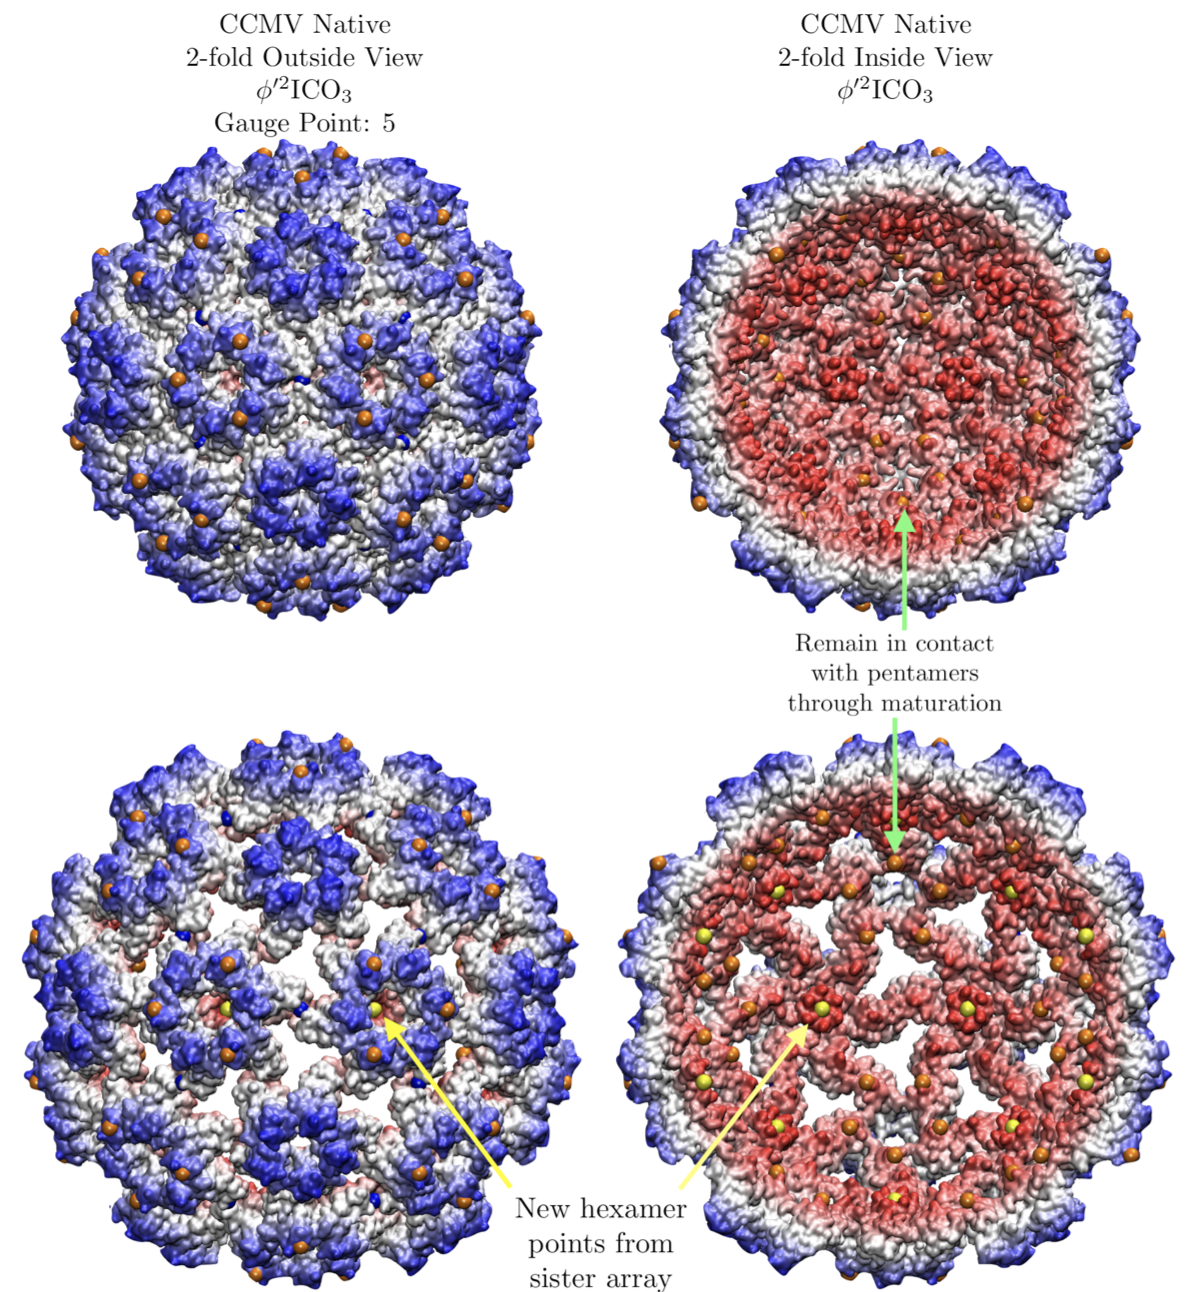
\includegraphics[width=0.5\textwidth]{images/CCMV_maturation.png}
	\caption{The above diagram shows CCMV in its native state (first row) and mature state (second row). Notice the points in orange are the points that characterize CCMV.}
	\label{fig:CCMV_maturation}
\end{figure}

\section{Mathematical View of the Problem}
To find a linear transformation that maps from native to mature point arrays while preserving, we solve matrix equations of the form \[TB_0 = B_1.\]
In this equation, \(B_0\) and \(B_1\) represent the native and mature point arrays respectively, and \(T\) is our desired linear transformation.\footnote{Recall that we realize icosahedral symmetry as a matrix group and icosahedral point arrays are sets of vectors, so it makes sense that we are solving a matrix equation.}
Since \(B_0\) and \(B_1\) are representatives of the point arrays, there exist many different equations of the form \(TB_0 = B_1\) that represent the same problem.
Therefore, we only need to find one equation of this form that is solvable.

In our example of CCMV, these equations will take the form \[T\cdot \begin{bmatrix}
    | & | \\
    \vec{t}_0 & \vec{v}_0 \\
    | & | \\
\end{bmatrix} = \begin{bmatrix}
    | & | \\
    \vec{t}_1 & \vec{v}_1 \\
    | & | \\
\end{bmatrix}\]
and we wish to find a choice of these four vectors such that the equation is solvable.

\subsection{Transitions Preserving Symmetry}
A transition \(T\) that preserves all of icosahedral symmetry must have the form: \begin{equation} \label{centralizer:ico}
T = \begin{bmatrix}
    z  & x  & -x & -x & x  & x \\
    x  & z  & x  & -x & -x & x \\
    -x & x  & z  & x  & -x & x \\
    -x & -x & x  & z  & x  & x \\
    x  & -x & -x & x  & z  & x \\
    x  & x  & x  & x  & x  & z
\end{bmatrix}\end{equation}

Our linear transformation \(T\) preserves icosahedral symmetry because it is in the centralizer of \(\mathcal{I}\) (or one its of maximal subgroups).
\begin{Definition}[Centralizer]
    The centralizer of a group \(G\), denoted by \(Z(G)\) is the set of elements that commute with all elements of \(G\).
    That is, \[Z(G) = \{z\ |\ gz = zg\ \forall g \in G\}.\]
\end{Definition}
Any matrix of the form given in equation \ref{centralizer:ico} is in \(Z(\mathcal{I})\), the centralizer of \(\mathcal{I}\).
Similar general matrix forms exist for matrices that are in \(Z(A_4)\), \(Z(D_{10})\), and \(Z(D_6)\). \cite{indelicatoetal2012}

\subsection{CCMV \(D_6\) Transition Example}
The following is an example of an equation for the CCMV virus the preserves \(D_6\) symmetry:
\begin{equation}
	\begin{bmatrix}
	    u  & w  & -w & x  & s  & s  \\
	    -t & y  & v  & -v & z  & -t \\
	    t  & v  & y  & v  & t  & -z \\
	    z  & -v & v  & y  & -t & -t \\
	    s  & x  & -w & w  & u  & s  \\
	    s  & w  & -x & w  & s  & u 
	\end{bmatrix}
	\cdot
	\begin{bmatrix}
	-1/2 & -3/2 \\
	-1/2 & 1/2 \\
	1/2 & -1/2 \\
	-1/2 & -1/2 \\
	-1/2 & 1/2 \\
	1/2 & 1/2
	\end{bmatrix} 
	=
	\begin{bmatrix}
	0 & 0 \\
	0 & 0 \\
	-1 & 0 \\
	0 & -1 \\
	0 & -1 \\
	0 & -1 \\
	\end{bmatrix}
	\label{eq:ccmv_d6_example}
\end{equation}
In this equation, the \( 6 \times 6 \) matrix on the left is the general form for linear transformations that preserve \( D_6 \) symmetry.
We have also chosen example vectors that generate the CCMV native and mature point arrays.

This equation is only one of many that represents a CCMV \( D_6 \) transition.
In order to compute how many of these equations exist, we simply need to mutiply the sizes of the icosahedral orbits of each vector individually.


\section{Computational Techniques}
In order to find a solvable equation (or say such an equation doesn't exist) of the form \(TB_0 = B_1\), we must search through up to hundreds of thousands of these equations.
This is infesible to do by hand, so we employ various programs to find solvable equations.

\subsection{Brute Force in C++}
As a first approach, I brute force every possible transitions matrix.
In order to do this, I take a set of values and create every possible transition matrix from those values.
If we take the set \(E = \{0, \pm\frac{1}{2}, \pm 1\}\) as the set of values, then for our example equation (see equation \ref{eq:ccmv_d6_example}), then there will be \(\abs{E}^8 = 390625\) possible transition matrices to check.
Because there are thousands of equations we need to check that look like our example, this approach quickly becomes infeasible.

\subsection{Equation Solving in Python}
The final approach to finding transitions is to use a linear matrix equation solver within the Python \texttt{sympy} package.
This package allows us to give it an equation such as equation \ref{eq:ccmv_d6_example} and it will tell us if a solution exists or not.
We can simply loop through all possible equations and give it to \texttt{sympy} and check if any have a solution.
If we find such an equation with a solution, then there exists a symmetry preserving transition.
If we cannot find any equation, then there does not exist any symmetry preserving transitions.

\subsection{Parallel Computing on Jigwé}
Since checking of each equation is an independent task, this problem is said to be \emph{embarassingly parallel}.
Therefore we can speed up computation by employing parallel computing.
Kalamazoo College has a supercomputer known as Jigwé (pronouced 'Cheekua' and is Potawatomi for Thunderbird) in which we can perform parallel computing.

\section{Conclusion}
By running my programs, I have produced the following results:
\begin{itemize}
    \item Reproduce \(D_6\) transitions for CCMV found in \cite{indelicatoetal2012}.
    \item I have figured out what symmetry preserving transitions exist between all of the 55 standard point arrays. Larger point arrays must be built from these 55, so this data also helps in determining what transitions are and are not possible between bigger point arrays.
    \item There cannot exist any transition that preserves all of icosahedral symmetry between different point arrays, since no such transition exists between any of the 55 standard point arrays.
\end{itemize}

\section{Future Directions}
As a final thought, a few future directions one could take with this research:
\begin{itemize}
    \item I have been solving these equations in 6 dimensions, but since we live in 3 dimensions, we could project these point arrays into 3 dimensions, using the projection matrix given in \cite{indelicatoetal2012}.
    Since multiple 6 dimensional transitions exist, it may be possible that they project onto the same transition in 3 dimensions.
    \item I could attempt to find all possible transitions between larger point arrays because even if a transition exists between all of its components, a transition may not exist for the larger point array.
\end{itemize}

\medskip
\bibliographystyle{unsrt}%Used BibTeX style is unsrt
\bibliography{references}

\end{document}